\documentclass[runningheads]{llncs}

% LNCS basic packages
\usepackage[T1]{fontenc}
\usepackage{graphicx}
\usepackage{amsmath,amssymb}
\usepackage{booktabs}
\usepackage{multirow}
\usepackage{hyperref}
\usepackage[table]{xcolor}
\usepackage{placeins}

% Convenience
\newcommand{\todo}[1]{\textcolor{red}{\textbf{[TODO: #1]}}}

\begin{document}

\title{Decoder-Only Topology-Aware Fine-Tuning of CT Foundation Models\\for Coronary Artery Segmentation}
\titlerunning{Decoder-Only Topology-Aware Fine-Tuning for Coronary Segmentation}

\author{First Author\inst{1}\orcidID{0000-0000-0000-0000} \and
Second Author\inst{1}\orcidID{0000-0000-0000-0000}}
%
\authorrunning{F. Author et al.}
%
\institute{University Name, City, Country \\
    \email{\{first,second\}@university.ac.uk}}

\maketitle

%----------------------------------------------------------------------
\begin{abstract}
Foundation models for CT segmentation achieve strong volumetric overlap through large-scale pretraining, but their adaptation for topology-sensitive tasks such as coronary artery segmentation remains under-studied.
We present a systematic study of how encoder adaptation strategy interacts with topology-aware supervision when fine-tuning CT-FM, a SegResNet foundation model pretrained on 148K CT scans.
On ImageCAS ($n{=}250$ test), we cross five adaptation strategies---decoder-only, BitFit, skip adapters, partial unfreeze, and full fine-tuning---with three loss weights for a previously proposed differentiable bifurcation connectedness (Soft BCS) surrogate, yielding an ablation grid of segmentation and topology metrics.
Decoder-only fine-tuning achieves strong overlap--connectivity balance with both Soft BCS (Dice~0.792, BCS~0.722) and clDice (Dice~0.794); full fine-tuning at matched learning rate achieves the best results (Dice~0.797--0.801, BCS~0.716--0.735) but is sensitive to LR---a 10$\times$ increase destroys pretrained features.
Centered Kernel Alignment confirms that parameter-efficient strategies preserve encoder representations (CKA${\geq}0.82$), while full fine-tuning moderately adapts them (CKA${\approx}0.75$), and that the adaptation strategy---not the loss function---is the primary determinant of success.
We further evaluate cross-domain transfer to ASOCA, where annotation protocol mismatch (full-tree vs.\ major-vessel labels) causes systematic over-segmentation (Dice~0.48, BCS~0.79).
The frozen encoder acts as a reusable topology-aware backbone: $k{=}1$ low-shot adaptation with aggressive decoder learning rate yields Dice~$0.704{\pm}0.028$ across replicate runs with random case selection, stabilised to 0.749 via soft ensembling (BCS~0.743), demonstrating that topology learned on the source domain transfers without requiring topology supervision on the target.
\keywords{Coronary artery segmentation \and Foundation models \and Topology-aware learning \and Low-shot adaptation \and Encoder adaptation}
\end{abstract}

%----------------------------------------------------------------------
\section{Introduction}

Foundation models pretrained on large-scale CT data offer strong initialisation for downstream segmentation tasks, reducing the need for task-specific training from scratch~\cite{pai_ctfm_2025,huang_stu_2023}.
In coronary artery segmentation, accurate delineation underpins stenosis quantification, FFR-CT estimation, and stent planning~\cite{lin_deep_2022}.
However, two practical challenges limit straightforward deployment of pretrained models.

First, \emph{how to adapt} the pretrained encoder is an open question.
Full fine-tuning risks catastrophic forgetting of pretrained features, while freezing the encoder entirely may under-utilise its capacity.
The transfer-learning literature in NLP and 2D vision has studied parameter-efficient strategies---BitFit~\cite{zaken_bitfit_2022}, adapters~\cite{houlsby_adapters_2019}, partial unfreezing~\cite{lee_surgical_2023}---but their interaction with \emph{topology-aware losses} in 3D medical imaging is unexplored.

Second, \emph{annotation protocol mismatch} between source and target datasets creates a distribution shift in label space.
A model pretrained on full coronary tree annotations (ImageCAS~\cite{zeng_imagecas_2023}) will systematically over-segment when applied to datasets labelling only major vessels (ASOCA~\cite{gharleghi_asoca_2022}).
This is not domain shift in image appearance but a mismatch in the definition of the target structure.
In the low-shot regime, where few labelled examples are available, topology-aware supervision may act as an inductive bias to constrain the solution space~\cite{shit_cldice_2021,hu_topology_2019,clough_topological_2022}.

We address both challenges in a unified study.
On ImageCAS ($n{=}638$ train, $n{=}250$ test), we systematically ablate five encoder adaptation strategies crossed with three topology loss weights, using the differentiable Soft BCS loss that directly supervises branch-level connectivity at bifurcation points.
We complement the ablation with representational analysis (CKA similarity~\cite{kornblith_cka_2019} and linear probing) to explain \emph{why} certain strategies succeed.
We then evaluate cross-domain transfer to ASOCA under annotation protocol mismatch, testing whether the best adaptation strategy generalises and whether topology-aware supervision improves low-shot sample efficiency.

\paragraph{Contributions.}
\begin{enumerate}
    \item A systematic ablation of five encoder adaptation strategies $\times$ topology loss weights (Soft BCS and clDice), showing that adaptation strategy---not loss choice---determines fine-tuning success.
    \item Representational analysis (CKA, linear probing) showing that all parameter-efficient strategies preserve encoder features (CKA${\geq}0.82$), that full fine-tuning at matched learning rate moderately adapts them (CKA${\approx}0.75$ at the bottleneck), and that learning rate---not fine-tuning per se---determines whether pretrained representations survive.
    \item Cross-domain evaluation on ASOCA demonstrating that the frozen encoder acts as a reusable topology-aware backbone, enabling effective low-shot adaptation under annotation protocol mismatch.
\end{enumerate}

%----------------------------------------------------------------------
\section{Related Work}

\paragraph{Foundation model adaptation.}
Large pretrained models can be adapted via full fine-tuning, linear probing, or parameter-efficient methods including BitFit (bias-only tuning)~\cite{zaken_bitfit_2022}, bottleneck adapters~\cite{houlsby_adapters_2019,chen_adaptformer_2022}, and surgical fine-tuning of selected layers~\cite{lee_surgical_2023}.
Kumar et al.~\cite{kumar_finetuning_2022} showed that full fine-tuning can distort pretrained features and degrade out-of-distribution performance.
In medical imaging, STU-Net~\cite{huang_stu_2023} and CT-FM~\cite{pai_ctfm_2025} demonstrate scalable pretraining, but downstream adaptation strategies remain under-explored, particularly for topology-sensitive losses.

\paragraph{Topology-aware segmentation.}
clDice~\cite{shit_cldice_2021} penalises centreline disconnections via soft skeletonisation.
Persistent homology losses~\cite{clough_topological_2022,hu_topology_2019} target Betti numbers but are computationally expensive for 3D volumes.
Roug\'e et al.~\cite{rouge_topology_2024} combine topology-aware cascaded U-Nets for cerebrovascular segmentation.
The bifurcation connectedness score (BCS) and its differentiable Soft BCS surrogate directly supervise branch-level connectivity at bifurcation points (Section~\ref{sec:bcs}).
All prior topology work focuses on \emph{loss design}; none studies how the choice of \emph{adaptation strategy} interacts with topology-aware objectives.

%----------------------------------------------------------------------
\section{Methods}

\subsection{Background: BCS and Soft BCS Loss}
\label{sec:bcs}

We briefly review the bifurcation connectedness score (BCS) and its differentiable surrogate.
BCS evaluates whether predicted segmentations preserve connectivity at ground-truth bifurcation points.
Given a ground-truth skeleton, bifurcation voxels (degree ${\geq}3$) are clustered into junctions.
For each junction, branch stubs of length $l{=}8$ are traced along each outgoing branch.
A junction is \emph{preserved} if all its stubs are mutually reachable through the predicted segmentation (dilated skeleton, tolerance $\tau{=}3$).
BCS is the fraction of preserved junctions.

The differentiable Soft BCS loss operates on precomputed ground-truth stub labels.
Writing $p(v)$ for the predicted foreground probability at voxel $v$ and $\bar{p}_k = \frac{1}{|s_k|}\sum_{v \in s_k} p(v)$ for the mean probability on stub~$k$, the per-bifurcation loss uses a softmin weighting:
\begin{equation}\label{eq:softbcs}
\ell_c = 1 - \sum_k w_k \bar{p}_k, \quad
w_k = \frac{\exp(-\bar{p}_k/T)}{\sum_j \exp(-\bar{p}_j/T)},
\end{equation}
where $T{=}0.1$ concentrates gradients on the least-connected branch.
The total loss averages over all bifurcations in the training patch:
$\mathcal{L}_{\mathrm{softBCS}} = \frac{1}{|\mathcal{C}'|}\sum_{c \in \mathcal{C}'} \ell_c$.

\subsection{Base Model and Training Setup}

We use CT-FM~\cite{pai_ctfm_2025}, a SegResNet~\cite{myronenko_segresnet_2019} encoder (${\sim}$78M parameters) pretrained on 148K CT scans via self-supervised learning.
All experiments start from an ImageCAS-pretrained checkpoint that was fine-tuned with a multi-task loss combining DiceCE segmentation and Frangi vesselness prediction~\cite{frangi_multiscale_1998} (denoted $\mathcal{L}_v$, our ``L1'' baseline).
The composite training loss is:
\begin{equation}\label{eq:loss}
\mathcal{L} = \mathcal{L}_v + \lambda_s \, \mathcal{L}_{\mathrm{topo}},
\end{equation}
where $\mathcal{L}_{\mathrm{topo}}$ is either $\mathcal{L}_{\mathrm{softBCS}}$ or $\mathcal{L}_{\mathrm{clDice}}$~\cite{shit_cldice_2021}, and $\lambda_s$ controls the topology loss weight.
Training uses ImageCAS~\cite{zeng_imagecas_2023} (638 train, 112 val, 250 test), $96^3$ patches with random pos/neg cropping, 30 epochs, and learning rate reduced on plateau (factor 0.5, patience 5 epochs).

\subsection{Adaptation Strategies}
\label{sec:strategies}

We evaluate five strategies spanning a parameter-efficiency spectrum (Table~\ref{tab:strategies}).
All start from the same L1 checkpoint and use identical data augmentation, differing only in which parameters are trainable and the learning rate (Table~\ref{tab:strategies}).

\begin{table}[t]
\caption{Encoder adaptation strategies. All share the same 10M-parameter decoder.}
\label{tab:strategies}
\centering
\small
\begin{tabular}{llrr}
\toprule
Strategy & Encoder trainable params & Total trainable & LR \\
\midrule
Frozen (decoder-only)     & 0                        & 10.0M  & $10^{-5}$ \\
BitFit (norm params)      & ${\sim}$14K (BN bias+scale) & 10.0M  & $10^{-5}$ \\
Adapters (skip bottleneck)& ${\sim}$175K              & 10.2M  & $10^{-5}$ \\
Partial (last enc.\ block) & 17.7M                   & 27.7M  & $5{\times}10^{-5}$ \\
Full (all parameters)     & 77.8M                    & 87.8M  & $10^{-5}$ \\
\bottomrule
\end{tabular}
\end{table}

Each strategy is crossed with $\lambda_s \in \{0.03, 0.05, 0.10\}$.
BitFit and adapter experiments are run at $\lambda_s{=}0.05$ only; full fine-tuning at $\lambda_s{=}0.10$ only.
Together with two clDice comparisons (frozen and full at matched settings), this yields 11 experimental cells plus the L1 baseline ($\lambda_s{=}0$).

\subsection{Representational Analysis}

To understand \emph{why} certain strategies preserve performance, we measure how much the encoder changes during fine-tuning.

\paragraph{CKA similarity~\cite{kornblith_cka_2019}.}
We compute linear Centered Kernel Alignment between the L1 baseline encoder and each fine-tuned encoder at five resolution levels (32ch/96$^3$ to 512ch/6$^3$).
CKA${\approx}1$ indicates preserved representations; low CKA indicates feature drift.

\paragraph{Linear probing.}
We probe whether bifurcation-discriminative information is linearly accessible at each network level.
Ground-truth skeleton voxels within $\tau{=}3$ voxels of a bifurcation point (skeleton voxel with ${\geq}3$ neighbours under 26-connectivity) are labelled positive; remaining skeleton voxels are negative.
For each frozen checkpoint, we extract the feature vector at each labelled voxel by indexing into the encoder or decoder feature map at the corresponding (downsampled) spatial location, using sliding-window inference (96$^3$ patches, 50\% overlap) to cover full volumes.
We sample 500 voxels per class per case (30 train, 20 val) and fit an L2-regularised logistic regression (scikit-learn, $C{=}1.0$, LBFGS).
Higher probe AUC at a given level indicates that bifurcation-relevant features are linearly separable there.

\subsection{Cross-Domain Transfer: ASOCA}
\label{sec:asoca}

ASOCA~\cite{gharleghi_asoca_2022} provides 40 CTCA scans (20 normal, 20 diseased) with major-vessel-only annotations, contrasting ImageCAS's full coronary tree labels.
This annotation protocol mismatch means the pretrained model systematically includes side branches absent from ASOCA's ground truth.

\paragraph{Zero-shot evaluation.}
We apply all ImageCAS-trained models directly to ASOCA (threshold 0.5) to quantify the mismatch.

\paragraph{Low-shot fine-tuning.}
We fine-tune using $k \in \{1, 5, 10\}$ labelled ASOCA scans per group ($2k$ total).
The encoder and first two decoder levels are frozen, adapting only the last two decoder levels---motivated by the insight that the model needs to suppress side branches rather than learn new features.
We sweep the learning rate across three orders of magnitude ($5{\times}10^{-6}$ to $5{\times}10^{-4}$) and the binarisation threshold $t \in [0.3, 0.9]$.
For $k{\geq}5$, we additionally evaluate dropout regularisation ($p{=}0.2$) to prevent overfitting with increased training data.
We report results at the optimal configuration per $k$.

\subsection{Evaluation Metrics}

We report Dice (volumetric overlap), clDice~\cite{shit_cldice_2021} (centreline overlap), BCS (bifurcation connectedness, $\tau{=}3$, $l{=}8$; Section~\ref{sec:bcs}), HD95 (95th-percentile Hausdorff distance, mm), and Betti$_0$ error ($|\beta_0(P) - \beta_0(G)|$, connected component mismatch).

%----------------------------------------------------------------------
\section{Results}

\subsection{ImageCAS Ablation: Adaptation Strategy $\times$ BCS Weight}

Table~\ref{tab:ablation} presents the full ablation grid on $n{=}250$ ImageCAS test cases.

\begin{table}[t]
\caption{Ablation grid on ImageCAS ($n{=}250$ test). Best per-column in \textbf{bold}. Bottom rows compare clDice as an alternative topology loss. All inference at overlap$\,{=}\,$0.75. Significance vs.\ L1 baseline (paired bootstrap, $n{=}10{,}000$): $^{***}p{<}0.001$, $^{*}p{<}0.05$.}
\label{tab:ablation}
\centering
\small
\begin{tabular}{llcccccc}
\toprule
Adaptation & $\lambda_s$ & LR & Dice $\uparrow$ & clDice $\uparrow$ & BCS $\uparrow$ & HD95\,(mm) $\downarrow$ & Betti$_0$ $\downarrow$ \\
\midrule
\multicolumn{2}{l}{\textit{L1 baseline ($\lambda_s{=}0$)}} & $10^{-4}$ & 0.792 & 0.869 & 0.688 & \textbf{6.7} & 5.02 \\
\midrule
\multirow{3}{*}{Frozen}
 & 0.03 & $10^{-5}$ & 0.794$^{***}$ & 0.864 & 0.705$^{***}$ & 7.2 & 6.81 \\
 & 0.05 & $10^{-5}$ & 0.792 & 0.856 & 0.722$^{***}$ & 8.8 & 9.11 \\
 & 0.10 & $10^{-5}$ & 0.785 & 0.844 & 0.730$^{***}$ & 10.2 & 13.20 \\
\midrule
\multirow{3}{*}{Partial}
 & 0.03 & $5{\times}10^{-5}$ & 0.793 & 0.858 & 0.715$^{***}$ & 9.4 & 8.44 \\
 & 0.05 & $5{\times}10^{-5}$ & 0.792 & 0.862 & 0.719$^{***}$ & 7.8 & 8.19 \\
 & 0.10 & $5{\times}10^{-5}$ & 0.789 & 0.858 & 0.714$^{***}$ & 8.5 & 7.95 \\
\midrule
BitFit & 0.05 & $10^{-5}$ & 0.793 & 0.859 & 0.721$^{***}$ & 8.1 & 8.66 \\
Adapters & 0.05 & $10^{-5}$ & 0.790 & 0.852 & 0.714$^{***}$ & 9.3 & 10.56 \\
\midrule
Full & 0.10 & $10^{-5}$ & 0.797$^{***}$ & 0.866 & \textbf{0.735}$^{***}$ & \textbf{6.7} & 5.66 \\
\midrule
\multicolumn{8}{l}{\textit{Topology loss comparison: clDice~\cite{shit_cldice_2021}}} \\
Frozen (clDice) & 0.05 & $10^{-5}$ & 0.794$^{*}$ & 0.861 & 0.706$^{***}$ & 9.1 & 9.09 \\
Full (clDice) & 0.10 & $10^{-5}$ & \textbf{0.801}$^{***}$ & \textbf{0.872}$^{*}$ & 0.716$^{***}$ & 6.8 & \textbf{5.02} \\
\bottomrule
\end{tabular}
\end{table}

\paragraph{Effect of BCS weight.}
Within the frozen rows, increasing $\lambda_s$ monotonically raises BCS but progressively lowers Dice; partial rows follow a similar trend at low weights but BCS peaks at $\lambda_s{=}0.05$ and slightly reverses at $\lambda_s{=}0.10$ (0.719${\to}$0.714).
At $\lambda_s{=}0.03$, BCS improves by $+1.7$\,pp (frozen) to $+2.7$\,pp (partial) over L1 with a small Dice gain; at $\lambda_s{=}0.10$, frozen BCS reaches its peak ($+4.2$\,pp) but Dice drops by $0.3$--$0.7$\,pp.
Paired bootstrap tests ($n{=}10{,}000$ resamples) confirm that all BCS improvements are statistically significant ($p{<}0.001$), while Dice changes remain non-significant for most parameter-efficient strategies.
The sweet spot is $\lambda_s \in [0.03, 0.05]$.

\paragraph{Frozen vs.\ partial.}
Partial fine-tuning uses a higher LR ($5{\times}10^{-5}$) than frozen ($10^{-5}$) because unfreezing the last encoder block requires a stronger learning signal; this rate was selected via validation sweep and is consistent across all partial configurations.
At $\lambda_s{=}0.05$, frozen and partial strategies achieve nearly identical Dice ($0.0$\,pp difference) and BCS ($0.3$\,pp); partial offers slightly better HD95 (7.8 vs.\ 8.8\,mm) but the overall benefit is marginal.

\paragraph{Full fine-tuning.}
Full fine-tuning with Soft BCS at matched settings (LR$\,{=}\,10^{-5}$, 30 epochs, L1 initialisation) achieves Dice~0.797, the highest BCS of any configuration (0.735), and HD95~6.7\,mm---comparable to full fine-tuning with clDice (Dice~0.801, BCS~0.716, HD95~6.8\,mm).
Notably, an earlier run at 10$\times$ higher learning rate produced catastrophic overfitting (HD95${>}$30\,mm); CKA analysis (Table~\ref{tab:cka}) confirms this was a learning rate artefact rather than an inherent limitation of full fine-tuning.

\paragraph{Topology loss comparison.}
To disentangle the roles of adaptation strategy and loss function, we replace Soft BCS with clDice~\cite{shit_cldice_2021} at matched settings (same LR, epochs, and L1 initialisation).
At the frozen setting, clDice ($w{=}0.05$) achieves Dice~0.794, comparable to Soft BCS (0.792--0.794), with similar BCS (0.706 vs.\ 0.722).
Under full fine-tuning, both losses perform similarly: clDice achieves Dice~0.801 and BCS~0.716, while Soft BCS reaches Dice~0.797 and BCS~0.735.
Both full fine-tuning variants achieve significant improvements over L1 in both Dice and BCS ($p{<}0.001$, paired bootstrap); Full+clDice is also the only configuration to significantly improve the clDice metric itself ($p{=}0.022$).
The ${\leq}0.4$\,pp Dice difference and ${\leq}1.9$\,pp BCS difference confirm that the \emph{adaptation strategy} is the primary determinant of performance, with the specific topology loss playing a secondary role.

Figure~\ref{fig:scatter} visualises the change in Dice and BCS relative to the L1 baseline for all experimental cells.
All parameter-efficient strategies improve BCS ($+1.7$ to $+4.2$\,pp) with modest Dice cost (${\leq}0.2$\,pp at $\lambda_s{\leq}0.05$; up to $0.7$\,pp at $\lambda_s{=}0.10$).
Full fine-tuning achieves both higher Dice and higher BCS than parameter-efficient strategies: $+0.5$\,pp Dice / $+4.7$\,pp BCS (Soft BCS) and $+0.9$\,pp Dice / $+2.8$\,pp BCS (clDice).

\begin{figure}[t]
\centering

\includegraphics[width=0.95\linewidth]{../figures/fig1_dice_bcs_scatter.pdf}
\caption{Change in Dice and BCS relative to L1 baseline across all experimental cells. Parameter-efficient strategies improve BCS ($+1.7$ to $+4.2$\,pp) with modest Dice cost (${\leq}0.7$\,pp). Full fine-tuning achieves both higher Dice and BCS than parameter-efficient strategies. All BCS improvements are statistically significant ($p{<}0.001$, paired bootstrap).}
\label{fig:scatter}
\end{figure}

\subsection{CKA Similarity Analysis}

Table~\ref{tab:cka} shows CKA similarity between the L1 encoder and each fine-tuned encoder at five resolution levels.

\begin{table}[t]
\caption{CKA similarity to L1 baseline at each encoder level. Higher values indicate preserved representations. Parameter-efficient strategies maintain CKA${\geq}0.82$. Full fine-tuning at matched LR ($10^{-5}$) moderately adapts the encoder (CKA${\approx}$0.75 at bottleneck), while a 10$\times$ higher LR causes severe drift (CKA${=}$0.37).}
\label{tab:cka}
\centering
\small
\begin{tabular}{lccccc}
\toprule
 & \multicolumn{5}{c}{Encoder Level (channels, spatial resolution)} \\
\cmidrule(lr){2-6}
Strategy & 32ch, 96$^3$ & 64ch, 48$^3$ & 128ch, 24$^3$ & 256ch, 12$^3$ & 512ch, 6$^3$ \\
\midrule
Frozen ($\lambda_s{=}0.05$)  & 1.00 & 0.99 & 0.99 & 0.98 & 0.88 \\
BitFit ($\lambda_s{=}0.05$)  & 1.00 & 0.99 & 0.99 & 0.98 & 0.89 \\
Adapter ($\lambda_s{=}0.05$) & 1.00 & 0.99 & 0.99 & 0.97 & \textbf{0.90} \\
Partial ($\lambda_s{=}0.05$) & 1.00 & 0.99 & 0.99 & 0.97 & 0.84 \\
\midrule
Full+BCS ($\lambda_s{=}0.10$, LR$\,{=}\,10^{-5}$)    & 1.00 & 0.97 & 0.95 & 0.92 & 0.75 \\
Full+clDice ($w{=}0.10$, LR$\,{=}\,10^{-5}$)          & 1.00 & 0.97 & 0.95 & 0.92 & 0.76 \\
\rowcolor{gray!15}
\textit{Full (LR$\,{=}\,10^{-4}$)$^\dagger$}            & 0.95 & 0.74 & 0.67 & 0.44 & 0.37 \\
\bottomrule
\multicolumn{6}{l}{\footnotesize $^\dagger$\,Initial run with 10$\times$ higher LR; shown as cautionary comparison.} \\
\end{tabular}
\end{table}

All parameter-efficient strategies maintain CKA${\geq}0.82$ at every level, confirming that the pretrained encoder already contains topology-relevant representations.
Full fine-tuning at matched LR ($10^{-5}$) produces moderate encoder adaptation: CKA remains above 0.92 at levels 0--3 and drops to ${\approx}$0.75 at the bottleneck---sufficient to improve Dice by $+0.5$--$0.9$\,pp without destroying pretrained features.
Critically, both Full+BCS and Full+clDice show nearly identical CKA profiles (0.75 vs.\ 0.76 at bottleneck), confirming that the topology loss does not differentially affect encoder representations.
The earlier confounded run (LR$\,{=}\,10^{-4}$) shows CKA collapsing to 0.37 at the bottleneck, demonstrating that learning rate---not full fine-tuning per se---determines whether pretrained representations are preserved.
Figure~\ref{fig:cka} visualises this three-tier structure: parameter-efficient strategies (CKA${\geq}$0.82), matched full fine-tuning (CKA${\approx}$0.75), and LR-confounded full fine-tuning (CKA${=}$0.37).

\begin{figure}[t]
\centering

\includegraphics[width=0.85\linewidth]{../figures/fig1_cka_heatmap.pdf}
\caption{How much does fine-tuning change the encoder? Parameter-efficient strategies (top three rows) maintain CKA${\geq}$0.84 throughout. Full fine-tuning at matched LR ($10^{-5}$; rows 4--5) moderately adapts the bottleneck (CKA${\approx}$0.75). The confounded run (LR$\,{=}\,10^{-4}$; bottom row) shows progressive degradation, reaching CKA${=}$0.37 at the deepest level.}
\label{fig:cka}
\end{figure}

\subsection{Linear Probing: Encoder and Decoder}

Table~\ref{tab:probe} reports bifurcation detection AUC from linear probes on frozen encoder and decoder features.

\begin{table}[t]
\caption{Linear probe AUC for bifurcation detection at each encoder and decoder level. \textbf{Bold}: highest AUC per model. All strategies---including full fine-tuning at matched LR---peak at encoder level~1.}
\label{tab:probe}
\centering
\small
\begin{tabular}{lccccc}
\toprule
 & \multicolumn{5}{c}{Encoder Level (AUC)} \\
\cmidrule(lr){2-6}
Model & 32ch, 96$^3$ & 64ch, 48$^3$ & 128ch, 24$^3$ & 256ch, 12$^3$ & 512ch, 6$^3$ \\
\midrule
L1 baseline             & 0.684 & \textbf{0.813} & 0.772 & 0.705 & 0.620 \\
Frozen ($\lambda_s{=}0.05$)  & 0.686 & \textbf{0.811} & 0.763 & 0.705 & 0.623 \\
BitFit ($\lambda_s{=}0.05$)  & 0.687 & \textbf{0.812} & 0.765 & 0.706 & 0.621 \\
Adapter ($\lambda_s{=}0.05$) & 0.687 & \textbf{0.811} & 0.763 & 0.705 & 0.614 \\
Partial ($\lambda_s{=}0.05$) & 0.687 & \textbf{0.811} & 0.763 & 0.700 & 0.602 \\
\midrule
Full+BCS ($\lambda_s{=}0.10$)   & 0.692 & \textbf{0.808} & 0.775 & 0.708 & 0.609 \\
Full+clDice ($w{=}0.10$)        & 0.691 & \textbf{0.817} & 0.776 & 0.711 & 0.631 \\
\rowcolor{gray!15}
\textit{Full (LR$\,{=}\,10^{-4}$)$^\dagger$} & 0.680 & 0.773 & \textbf{0.794} & 0.694 & 0.638 \\
\midrule
 & \multicolumn{4}{c}{Decoder Level (AUC)} & \\
\cmidrule(lr){2-5}
 & 256ch, 12$^3$ & 128ch, 24$^3$ & 64ch, 48$^3$ & 32ch, 96$^3$ & \\
\midrule
L1 baseline             & 0.670 & 0.710 & \textbf{0.760} & 0.705 & \\
Frozen ($\lambda_s{=}0.05$)  & 0.667 & 0.710 & \textbf{0.756} & 0.690 & \\
BitFit ($\lambda_s{=}0.05$)  & 0.669 & 0.712 & \textbf{0.758} & 0.690 & \\
Adapter ($\lambda_s{=}0.05$) & 0.676 & 0.708 & \textbf{0.755} & 0.694 & \\
Partial ($\lambda_s{=}0.05$) & 0.669 & 0.708 & \textbf{0.750} & 0.692 & \\
\midrule
Full+BCS ($\lambda_s{=}0.10$)   & 0.692 & 0.726 & \textbf{0.755} & 0.698 & \\
Full+clDice ($w{=}0.10$)        & 0.685 & 0.739 & \textbf{0.760} & 0.693 & \\
\rowcolor{gray!15}
\textit{Full (LR$\,{=}\,10^{-4}$)$^\dagger$} & 0.676 & \textbf{0.766} & 0.754 & 0.665 & \\
\bottomrule
\multicolumn{6}{l}{\footnotesize $^\dagger$\,Initial run with 10$\times$ higher LR; shown as cautionary comparison.} \\
\end{tabular}
\end{table}

In the encoder, all strategies---including full fine-tuning at matched LR---peak at level~1 (64ch, 48$^3$; AUC${\approx}$0.81), identical to the L1 baseline, confirming preserved bifurcation-discriminative features.
Only the confounded run (LR$\,{=}\,10^{-4}$) shifts the peak to level~2, consistent with the CKA finding that learning rate determines representation preservation.
In the decoder, all models peak at level~2 (AUC${\approx}$0.75--0.76); the similarity across decoder probes suggests that topology-aware losses refine how bifurcation information is routed to the output rather than relocating it within the network.

\subsection{ASOCA: Zero-Shot Transfer under Protocol Mismatch}
\label{sec:asoca_results}

Table~\ref{tab:zeroshot} reports zero-shot performance on ASOCA ($N{=}40$).

\begin{table}[t]
\caption{Zero-shot transfer to ASOCA ($N{=}40$). ImageCAS-pretrained models over-segment: high BCS (branches preserved) but low Dice (side branches penalised by major-vessel GT). Higher $\lambda_s$ increases BCS but further reduces Dice.}
\label{tab:zeroshot}
\centering
\small
\begin{tabular}{llccccc}
\toprule
Adaptation & $\lambda_s$ & Dice $\uparrow$ & clDice $\uparrow$ & BCS $\uparrow$ & HD95\,(mm) $\downarrow$ & Betti$_0$ $\downarrow$ \\
\midrule
\multicolumn{2}{l}{\textit{L1 baseline ($\lambda_s{=}0$)}} & \textbf{0.481} & \textbf{0.759} & 0.794 & \textbf{15.7} & \textbf{7.1} \\
\midrule
\multirow{3}{*}{Frozen}
 & 0.03 & 0.450 & 0.725 & 0.827 & 19.8 & 12.1 \\
 & 0.05 & 0.446 & 0.720 & 0.824 & 21.1 & 13.8 \\
 & 0.10 & 0.430 & 0.695 & 0.838 & 25.9 & 21.4 \\
\midrule
BitFit & 0.05 & 0.454 & 0.731 & \textbf{0.840} & 18.3 & 8.9 \\
Adapter & 0.05 & 0.454 & 0.730 & 0.835 & 20.0 & 12.4 \\
\midrule
\multirow{3}{*}{Partial}
 & 0.03 & 0.453 & 0.726 & 0.815 & 22.6 & 14.5 \\
 & 0.05 & 0.426 & 0.714 & 0.821 & 22.5 & 15.4 \\
 & 0.10 & 0.446 & 0.724 & 0.830 & 20.4 & 14.4 \\
\midrule
Full & 0.10 & 0.423 & 0.650 & 0.831 & 43.0 & 21.6 \\
\bottomrule
\end{tabular}
\end{table}

All models achieve high BCS (${\geq}0.79$) on ASOCA despite low Dice (${\leq}0.49$), confirming systematic over-segmentation due to annotation protocol mismatch rather than image-domain shift: the models predict too \emph{much} rather than too little.
Higher $\lambda_s$ further increases BCS ($+4.4$\,pp for frozen $\lambda_s{=}0.10$) at the cost of Dice ($-5.1$\,pp), amplifying the mismatch.
A threshold sweep ($t \in [0.3, 0.9]$) reveals that BCS remains remarkably stable (${\pm}2$\,pp) while Dice improves monotonically with higher thresholds.
At $t{=}0.9$, L1 recovers $+19$\,pp Dice while BCS remains stable (${\pm}2$\,pp).
Importantly, L1 outperforms all BCS-trained models at every threshold on ASOCA---BCS training reinforces branch preservation, which is precisely the opposite of what major-vessel-only annotations require.
Figure~\ref{fig:threshold} shows the threshold sweep; full per-model results appear in Supplementary~\S5. Normal cases show lower Dice than diseased due to more extensive side-branch over-segmentation, while diseased cases show higher HD95 (Supplementary~\S6).

\begin{figure}[t]
\centering

\includegraphics[width=\linewidth]{../figures/fig3_asoca_threshold.pdf}
\caption{Threshold calibration on ASOCA: a free lunch for protocol mismatch. \textbf{(a)}~Raising the binarisation threshold from 0.5 to 0.9 recovers $+19$\,pp Dice (green shading marks the improvement zone); L1 outperforms all BCS-trained models at every threshold. \textbf{(b)}~BCS remains stable across thresholds (${\pm}2$\,pp), confirming that overlap gains come at no connectivity cost.}
\label{fig:threshold}
\end{figure}

\subsection{ASOCA: Low-Shot Adaptation}

We fine-tune the L1 decoder on ASOCA with $k \in \{1, 5, 10\}$ scans per group (total $2k$ training cases), freezing the encoder and first two decoder levels.
This tests whether the frozen encoder serves as a \emph{reusable topology-aware backbone}---preserving bifurcation knowledge while the decoder adapts to ASOCA's major-vessel annotation protocol.

Learning rate is the dominant adaptation lever (Table~\ref{tab:lowshot}).
At the default LR ($5{\times}10^{-6}$), the decoder underfits; increasing LR to $5{\times}10^{-4}$ at $k{=}1$ yields Dice~0.748 and HD95~7.6\,mm---both substantially better than zero-shot (Dice~0.481, HD95~15.7\,mm)---while maintaining BCS~0.742.
However, replicate runs with random case selection show substantial variance (Dice~$0.704{\pm}0.028$, HD95~$30{\pm}15$\,mm), reflecting the sensitivity of $k{=}1$ to the specific training case.
Soft ensembling---averaging the probability maps of all 5 replicates before thresholding---recovers Dice to 0.749 (matching the best single run) with HD95~29.3\,mm, demonstrating that replicate variance can be tamed without additional labelled data.
Dropout trades marginal Dice ($-0.5$\,pp) for better connectivity (BCS~0.753).
At $k{=}5$ and $k{=}10$, dropout regularisation is necessary to prevent overfitting at high LR (Table~\ref{tab:lowshot}).

\begin{table}[t]
\caption{Low-shot fine-tuning on ASOCA. Encoder frozen; only the last two decoder levels are trainable. Two validation cases per group are held out for model selection; $n_{\mathrm{eval}}$ excludes both training and validation cases. All results at $t{=}0.5$; single best run per configuration shown. $^\ddagger$Mean$\pm$SD over replicate runs with random case selection. $^\S$Soft ensemble: averaged probability maps across 5 replicates before thresholding.}
\label{tab:lowshot}
\centering
\small
\begin{tabular}{cclcccc}
\toprule
$k$ & LR & Reg. & $n_{\mathrm{eval}}$ & Dice $\uparrow$ & BCS $\uparrow$ & HD95\,(mm) $\downarrow$ \\
\midrule
\multicolumn{3}{l}{\textit{Zero-shot ($t{=}0.5$)}} & 40 & 0.481 & 0.794 & 15.7 \\
\multicolumn{3}{l}{\textit{Zero-shot ($t{=}0.9$)}} & 40 & 0.671 & 0.801 & 13.0 \\
\midrule
1  & $5{\times}10^{-6}$ & ---  & 34 & 0.658 & 0.761 & 11.0 \\
1  & $5{\times}10^{-4}$ & ---  & 34 & \textbf{0.748} & 0.742 & \textbf{7.6} \\
1  & $5{\times}10^{-4}$ & dp   & 34 & 0.743 & \textbf{0.753} & 9.1 \\
\rowcolor{gray!8}
1$^\ddagger$  & $5{\times}10^{-4}$ & ---  & 34 & 0.704$\pm$.028 & 0.732$\pm$.039 & 30.2$\pm$14.6 \\
\rowcolor{gray!8}
1$^\S$  & $5{\times}10^{-4}$ & ---  & 34 & \underline{0.749} & \underline{0.743} & \underline{29.3} \\
\midrule
5  & $5{\times}10^{-6}$ & ---  & 26 & 0.687 & 0.672 & 24.1 \\
5  & $10^{-4}$          & dp   & 26 & \textbf{0.720} & \textbf{0.712} & \textbf{21.1} \\
\midrule
10 & $5{\times}10^{-6}$ & ---  & 16 & 0.680 & 0.733 & 44.0 \\
10 & $10^{-4}$          & dp   & 16 & \textbf{0.710} & \textbf{0.787} & \textbf{38.7} \\
\bottomrule
\end{tabular}
\end{table}

Figure~\ref{fig:lr_sweep} reveals a Dice--BCS dissociation across $k$ values.
At $k{=}1$, Dice rises monotonically with LR while BCS remains stable (${\sim}0.74$): overlap improves without sacrificing connectivity.
At $k{=}10$, the pattern reverses---Dice degrades at aggressive LR but BCS climbs to 0.819, the highest connectivity of any configuration.
This suggests that with more training data, aggressive LR overfits on volume but the frozen encoder still preserves junction structure.
Practically, $k{=}1$ offers the best balance of all three metrics (Dice, BCS, HD95).

\begin{figure}[t]
\centering
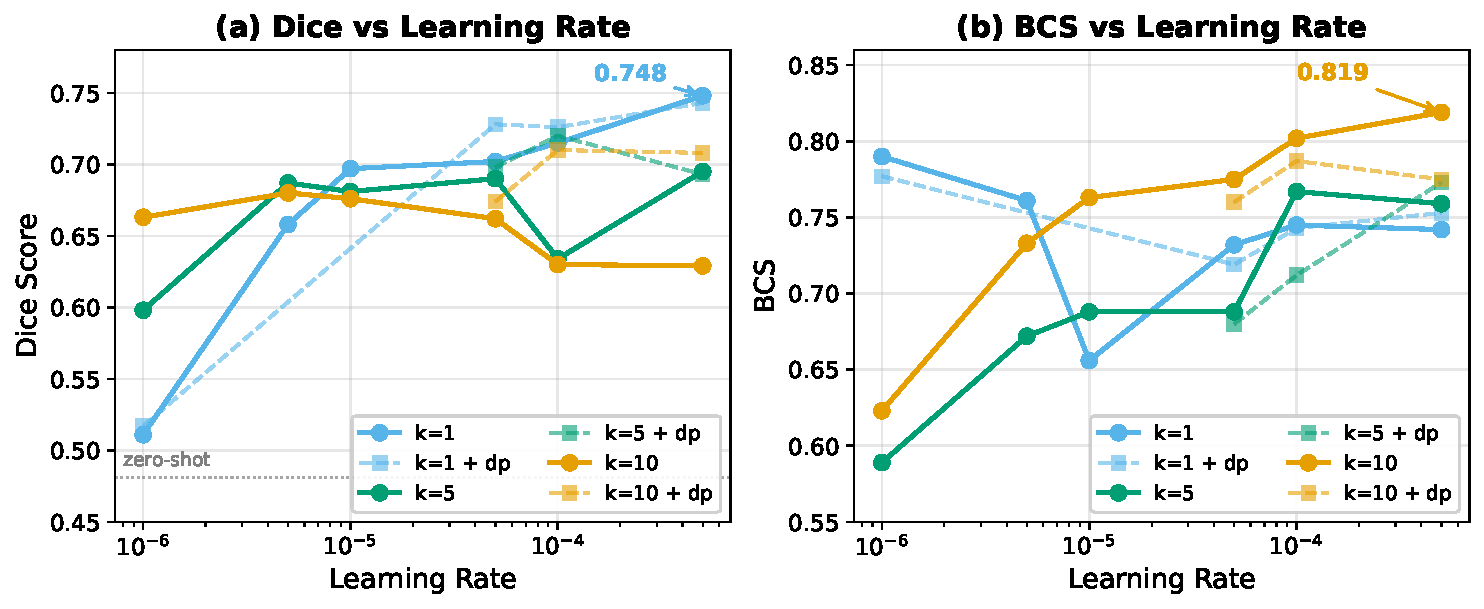
\includegraphics[width=\linewidth]{../figures/asoca_lr_sweep.pdf}
\caption{ASOCA low-shot performance vs.\ learning rate. \textbf{(a)}~At $k{=}1$, Dice rises monotonically with LR to 0.748. At $k{=}5{/}10$, Dice plateaus or drops without regularisation. \textbf{(b)}~BCS remains stable (${\sim}0.74$) at $k{=}1$ but increases with LR at $k{=}5{/}10$; $k{=}10$ reaches 0.819 even as its Dice degrades, revealing a Dice--BCS dissociation at higher $k$. Dashed lines: dropout regularisation (+dp).}
\label{fig:lr_sweep}
\end{figure}

The frozen encoder---not the loss function---drives this result.
Adding clDice during ASOCA fine-tuning ($w \in \{0.05, 0.10, 0.20\}$) is neutral (Dice~0.744--0.748, BCS~0.734--0.744), confirming that topology losses add nothing when the annotation protocol differs from the source domain.
Similarly, initialising from a BCS-trained decoder (EXP-048) hurts transfer (Dice~0.638), because BCS adapts the decoder to ImageCAS-specific branch topology that ASOCA does not share.
The mechanism is simple: the frozen encoder preserves bifurcation-level features, and aggressive decoder LR learns to suppress the side branches that ASOCA excludes.

Figure~\ref{fig:asoca_qual} illustrates the annotation protocol mismatch on a representative diseased case.
The zero-shot prediction includes side branches (blue) that are part of the full coronary tree but absent from ASOCA's major-vessel ground truth, explaining the high BCS but low Dice.
After $k{=}1$ fine-tuning with LR$\,{=}\,5{\times}10^{-4}$, the model learns to suppress side branches while preserving the major-vessel topology.

\begin{figure}[t]
\centering
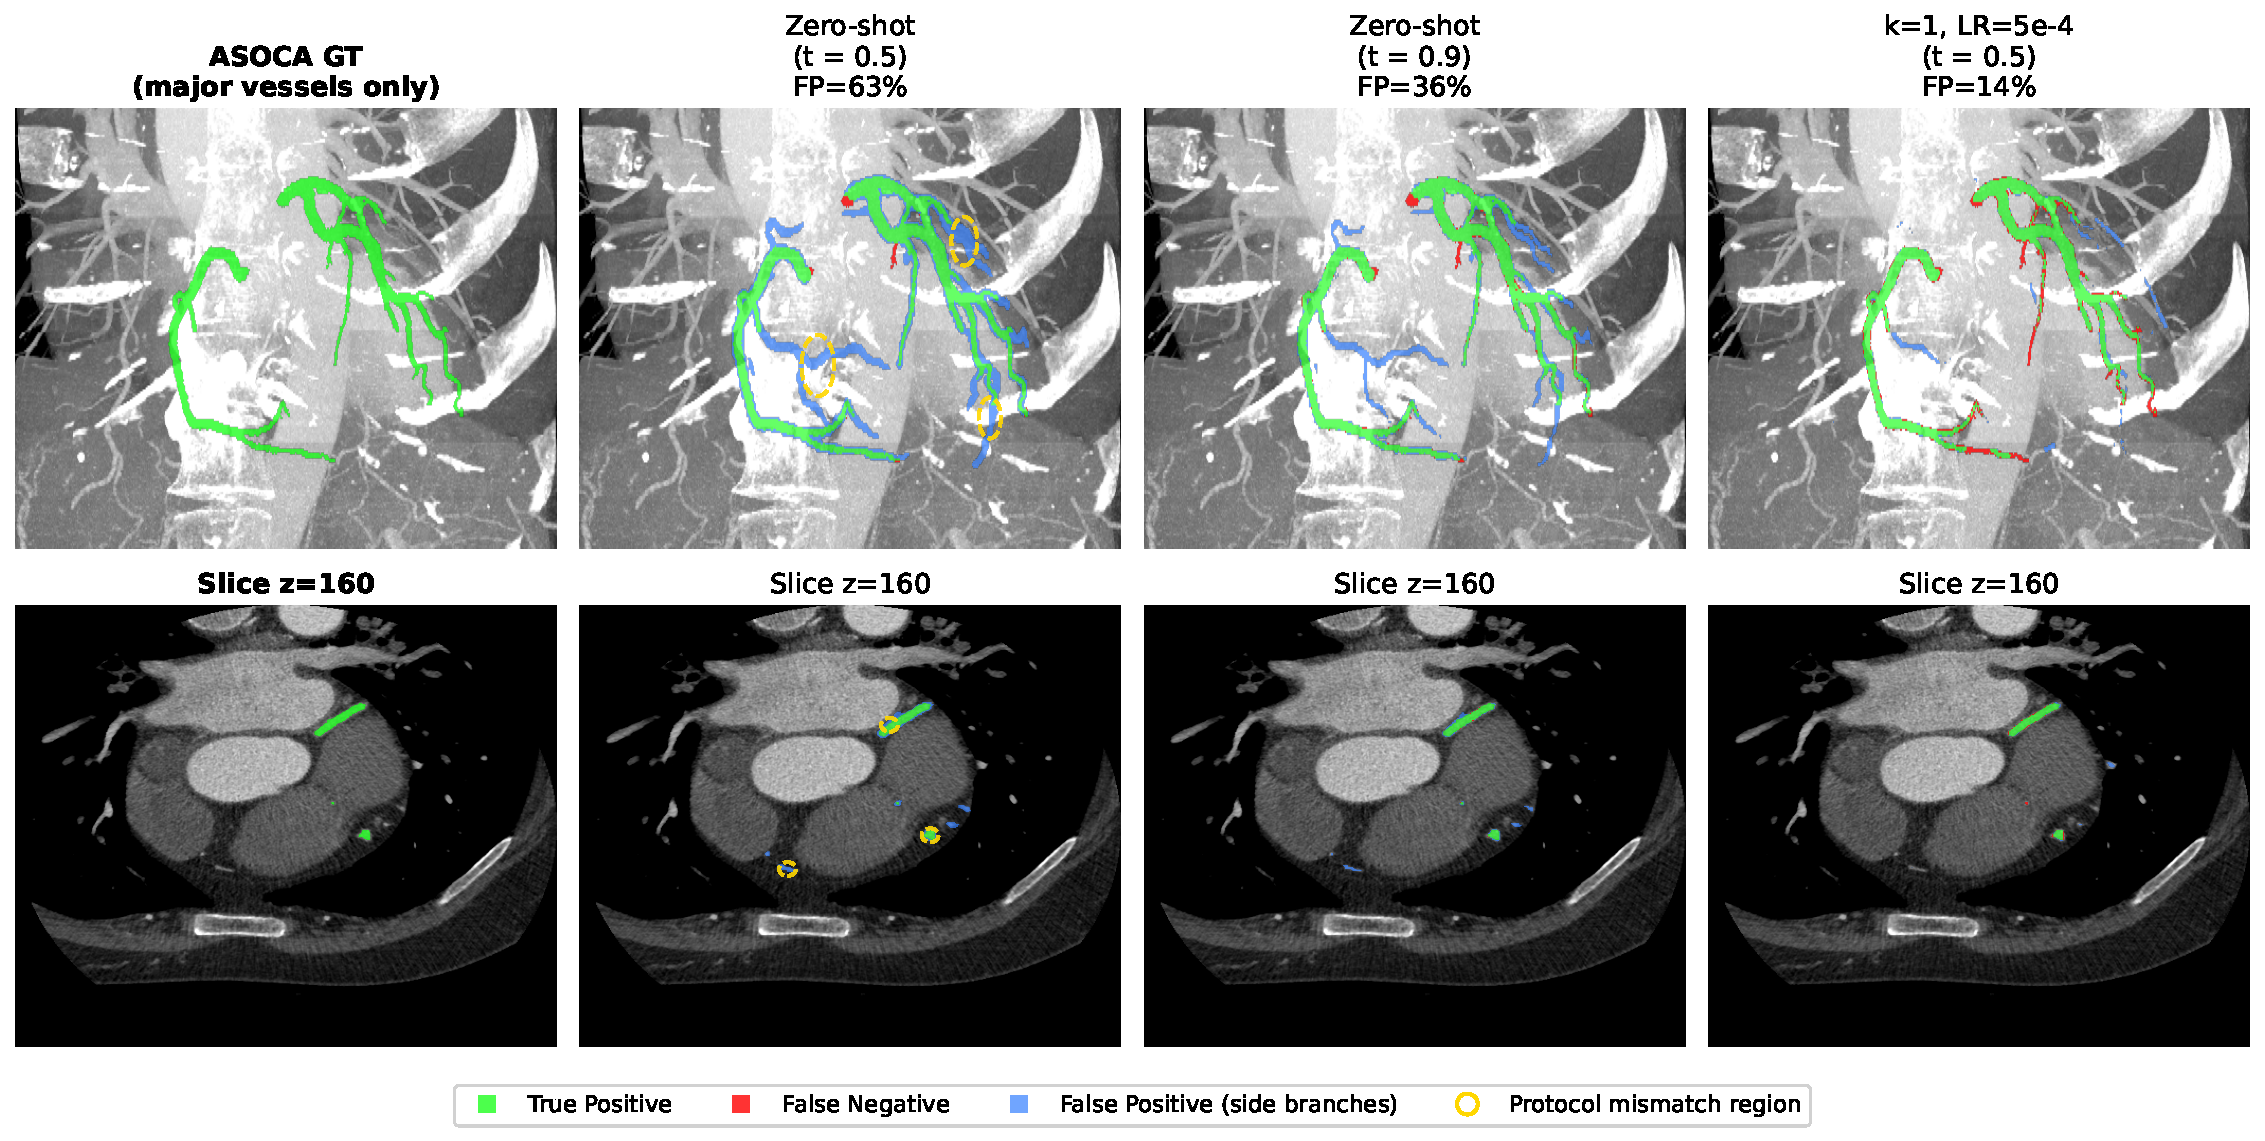
\includegraphics[width=\linewidth]{../figures/asoca_protocol_mismatch.pdf}
\caption{Annotation protocol mismatch on ASOCA (Diseased case 5). MIP projections (top) and axial slices (bottom). Green: true positive; red: false negative; blue: false positive (side branches present in the full coronary tree but absent from ASOCA's major-vessel annotations). Yellow circles highlight protocol mismatch regions. The frozen encoder preserves bifurcation knowledge while the decoder adapts: zero-shot (t\,{=}\,0.5) predicts the full tree (63\% FP); threshold calibration (t\,{=}\,0.9) suppresses side branches; $k{=}1$ fine-tuning (LR\,{=}\,$5{\times}10^{-4}$) reduces FP to 14\%.}
\label{fig:asoca_qual}
\end{figure}

%----------------------------------------------------------------------
\section{Discussion}

\paragraph{Adaptation strategy matters more than loss choice.}
The central finding is that encoder adaptation strategy---not the specific topology loss---determines fine-tuning success.
Decoder-only fine-tuning achieves strong connectivity--overlap balance with both Soft BCS (Dice~0.792, BCS~0.722) and clDice (Dice~0.794, BCS~0.706).
At the frozen setting, clDice and Soft BCS produce near-identical results, confirming that the adaptation strategy---not the loss---drives performance.
Full fine-tuning at matched LR ($10^{-5}$) achieves the best overall results (Dice~0.797--0.801, BCS~0.716--0.735) with moderate encoder adaptation (CKA${\approx}$0.75 at bottleneck), while the earlier confounded run (LR$\,{=}\,10^{-4}$) collapsed encoder representations (CKA${=}$0.37).
CKA and linear probing provide the mechanistic explanation: the pretrained encoder already encodes bifurcation-relevant features (probe AUC~0.81), and parameter-efficient strategies fully preserve them (CKA${\geq}0.82$); full fine-tuning moderately adapts them without destruction when LR is controlled.
$\lambda{=}0$ continued-training controls (Supplementary~\S1) confirm that the topology loss---not additional training epochs---drives the BCS gains.
This extends findings from NLP transfer learning~\cite{kumar_finetuning_2022} to 3D topology-aware medical image segmentation: full fine-tuning is viable when learning rate preserves pretrained representations.

\paragraph{BCS weight controls the overlap--connectivity trade-off.}
Within the frozen strategy, increasing $\lambda_s$ monotonically improves BCS at the cost of Dice and surface precision.
From $\lambda_s{=}0.03$ to $\lambda_s{=}0.10$, BCS improves by $+2.5$\,pp but Dice drops by $0.9$\,pp and HD95 increases by $+3.0$\,mm; partial follows a similar trend at low weights but BCS peaks at $\lambda_s{=}0.05$ and slightly reverses at $\lambda_s{=}0.10$.
This suggests a Pareto frontier that practitioners can navigate based on downstream requirements---higher $\lambda_s$ for connectivity-critical applications (FFR-CT, stent planning), lower $\lambda_s$ for volumetric and surface accuracy.

\paragraph{Frozen encoder as reusable topology-aware backbone.}
Zero-shot ASOCA transfer reveals high BCS (0.794) but low Dice (0.481): the encoder correctly identifies branches that ASOCA's major-vessel annotations exclude.
With just $k{=}1$ and aggressive decoder LR, the best single run recovers Dice~0.748 while maintaining BCS~0.742.
Topology losses (clDice) during ASOCA fine-tuning are neutral, confirming that the frozen encoder---not the loss---provides the topology prior.
Soft ensembling of replicates trained on different random case selections stabilises performance (Dice~0.749, matching the best single run) without additional labelled data---a practical strategy when low-shot variance is a concern.
The implication is that for cross-domain transfer with limited data, parameter-efficient adaptation preserves the topology prior encoded during source-domain training.

\paragraph{Limitations.}
This study evaluates a single foundation model (CT-FM SegResNet); supplementary material includes a comparison with three randomly-initialised architectures (STU-Net, SwinUNETR, MedNeXt) that confirms the foundation model advantage but does not test other pretrained backbones.
ASOCA's small size ($N{=}40$) limits statistical power for the low-shot analysis, and the $k{=}1$ result uses only 34 evaluation cases.
The Soft BCS formulation used here requires precomputed skeleton labels; a fully differentiable variant that computes stubs on-the-fly would remove this requirement.

%----------------------------------------------------------------------
\section{Conclusion}

We presented a systematic study of encoder adaptation strategies for topology-aware fine-tuning of a CT foundation model for coronary artery segmentation.
The adaptation strategy---not the choice of topology loss---is the primary determinant of fine-tuning success: decoder-only fine-tuning achieves strong overlap--connectivity balance with both Soft BCS (Dice~0.792, BCS~0.722) and clDice (Dice~0.794, BCS~0.706), preserving pretrained encoder features (CKA${\geq}0.82$).
Full fine-tuning at matched learning rate achieves the best same-domain results (Dice~0.797--0.801, BCS~0.716--0.735) with moderate encoder adaptation (CKA${\approx}$0.75), but requires careful LR selection---a 10$\times$ increase destroys pretrained representations (CKA${=}$0.37).
On ASOCA, annotation protocol mismatch causes systematic over-segmentation (Dice~0.48, BCS~0.79), but the frozen encoder serves as a reusable topology-aware backbone: $k{=}1$ adaptation with aggressive decoder learning rate yields Dice~$0.704{\pm}0.028$ across replicates, stabilised to 0.749 via soft ensembling (BCS~0.743).
The practical guideline is context-dependent: full fine-tuning for same-domain tasks with sufficient data, parameter-efficient adaptation for cross-domain transfer where preserving the topology prior is critical.

%----------------------------------------------------------------------
\begin{credits}
\subsubsection{\ackname}
This research was supported by [funder and project code to be disclosed upon publication].

\subsubsection{\discintname}
The authors have no competing interests to declare that are relevant to the content of this article.
\end{credits}

\bibliographystyle{splncs04}
\bibliography{references}

\end{document}
